\documentclass{article}

\usepackage[polish]{babel}
\usepackage[T1]{fontenc}
\usepackage{tabularx}
\usepackage{amsfonts}
\usepackage{amsmath}
\usepackage{mathtools}
\usepackage{enumitem}
\usepackage{graphicx}
\usepackage{algpseudocode}

\begin{document}
    \begin{titlepage}
        \title{Algorymy metaheurystyczne}
        \author{Mateusz Chęciński, Mateusz Tofil}
        \maketitle
    \end{titlepage}

    \section{Porównanie otoczeń: insert, invert, swap}

    W celu zbadania jakie otoczenie jest najlepsze z
    powyższych 3, przeprowadziliśmy eksperymenty wywołując
    metode ze zmienionym parametrem początkowym. Wszystkie
    eksperymetry były przeprowadzone dla tej samej instacji
    wraz z tym samym rozwiązaniem początkowym.

    \begin{figure}[h!]
        \centering
        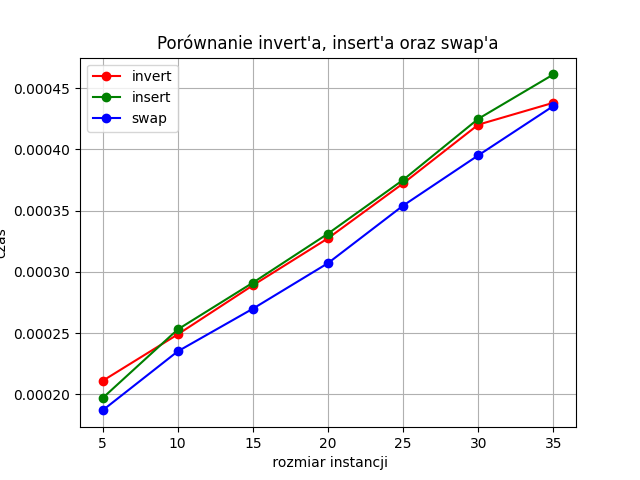
\includegraphics[width=11cm]{./spr2img/Figure_1.png}
        \caption{Porównanie otoczeń}
    \end{figure}

    Jak możemy zauważyć, dla wszystkich przeprowadzonych
    przez nas intacji, otocznie \emph{swap} okazało się być
    najelpszym. Pozostałe otoczenia, też nie są źle. Wszystkie
    otoczenia działają w czasie $\mathcal{O}(n)$ i różnią się tylko
    stałą, najmniejszą stałą posiada \emph{swap}

    \section{Czy długość listy Tabu ma znaczenie? }


\end{document}